\subsection{W-5}

MapReduce model: principy a jeho využití pro dotazování Big Data.

\subsubsection*{Definice}
MapReduce je programovací model a zpracovatelská technika pro distribuované výpočty, představená společností Google v roce 2004. Slouží ke zpracování a generování rozsáhlých datových sad pomocí paralelního algoritmu na clusteru počítačů.

\begin{itemize}
  \item Zpracování obrovských objemů dat (Big Data).
  \item Škálovatelnost na stovky až tisíce strojů.
  \item Skrytí složitosti paralelizace, odolnosti proti chybám, distribuce dat a vyvažování zátěže.
\end{itemize}

\subsubsection*{Architektura}
MapReduce se skládá z následujících procedur:

\begin{itemize}
  \item \textbf{Map:} Každý worker node aplikuje mapovací funkci na lokální data a zapisuje výstup do dočasného úložiště. Hlavní node zajišťuje, že pouze jedna kopie redundantních vstupních dat je zpracována.
  \item \textbf{Shuffle a sort:} Worker nody redistribuují data na základě výstupních klíčů (vygenerovaných mapovací funkcí), takže všechna data patřící jednomu klíči jsou umístěna na stejném worker nodu.
  \item \textbf{Reduce:} Worker nody nyní zpracovávají každou skupinu výstupních dat, podle klíče, paralelně.
\end{itemize}

\begin{figure}[H]
  \centering
  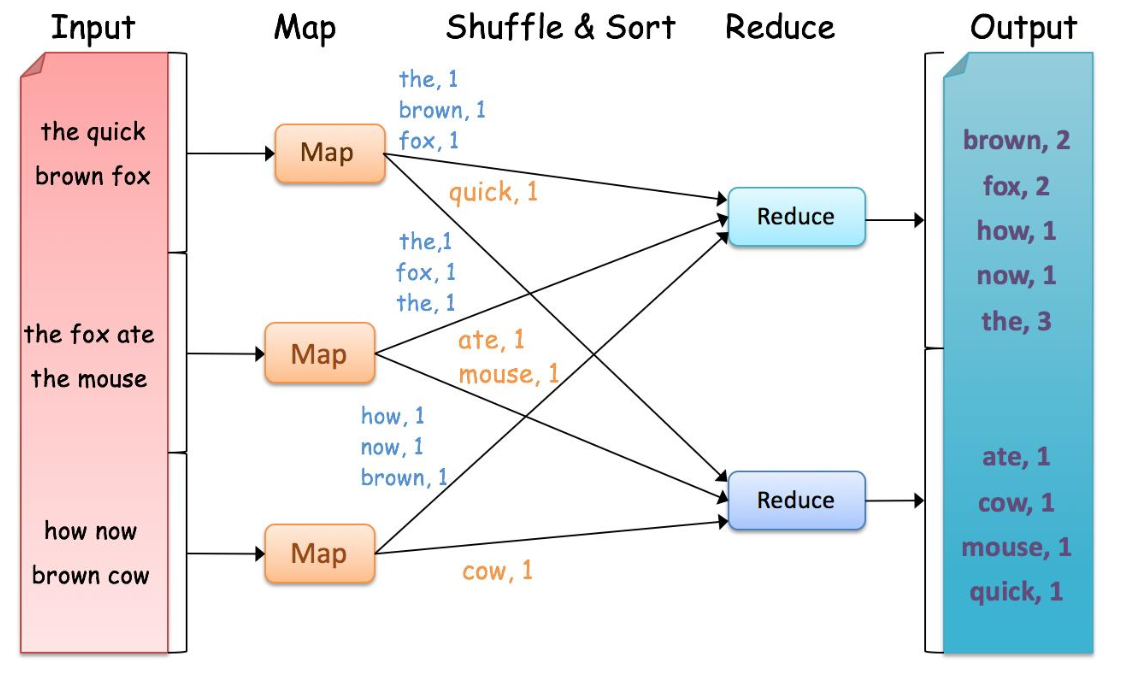
\includegraphics[width=0.8\textwidth]{img/map_reduce.png}
  \caption{MapReduce architektura}
\end{figure}

\subsubsection*{Základní pojmy v Hadoop}

%NODE = fyzický stroj/virtuální kontainer, kde běží JVM (Java Virtual Machine)
%● JOB = mapreduce program + konfigurace + vstupní data
%● ApplicationMaster = master, řídí výpočet
%● SPLIT = jednotná konečná část vstupu
%● TASK = slave, výpočet podle map/reduce funkce nad daty v 1 SPLITu
%● TASK ATTEMPT = pokus vypočíst 1 TASK na 1 NODU
%○ pokud node spadne -> framework předá TASK na jiný a vznikne nový attempt
%○ počet pokusů omezeno konfigurací -> JOB failed = map/reduce task attempts > max
%attempts
%● MAP = mapovací funkce (transformace, projekce, filtr, flatmap)
%● SHUFFLE = přesun dat z map fáze do reduce fáze (typicky po síti)
%● REDUCE = redukční funkce

\begin{itemize}
  \item \textbf{Node:} Fyzický stroj nebo virtuální kontejner, kde běží Java Virtual Machine (JVM).
  \item \textbf{Job:} MapReduce program, konfigurace a vstupní data.
  \item \textbf{Application Master:} Řídí výpočet.
  \item \textbf{Split:} Jednotná konečná část vstupu.
  \item \textbf{Task:} Výpočet podle map/reduce funkce nad daty v jednom splitu.
  \item \textbf{Task Attempt:} Pokus vypočítat jeden task na jednom nodu. Pokud node spadne, framework předá task jinému nodu a vznikne nový attempt. Počet pokusů je omezen konfigurací.
  \item \textbf{Map:} Mapovací funkce (transformace, projekce, filtr, flatmap).
  \item \textbf{Shuffle:} Přesun dat z map fáze do reduce fáze (typicky po síti).
  \item \textbf{Reduce:} Redukční funkce.
\end{itemize}

Důležité jsou optimalizace mimo samotný Map/Reduce algoritmus, jako například dělení na tasky, přidělování, vyvažování zátěže a nějaký error management.
